% Options for packages loaded elsewhere
\PassOptionsToPackage{unicode}{hyperref}
\PassOptionsToPackage{hyphens}{url}
%
\documentclass[
]{book}
\usepackage{lmodern}
\usepackage{amssymb,amsmath}
\usepackage{ifxetex,ifluatex}
\ifnum 0\ifxetex 1\fi\ifluatex 1\fi=0 % if pdftex
  \usepackage[T1]{fontenc}
  \usepackage[utf8]{inputenc}
  \usepackage{textcomp} % provide euro and other symbols
\else % if luatex or xetex
  \usepackage{unicode-math}
  \defaultfontfeatures{Scale=MatchLowercase}
  \defaultfontfeatures[\rmfamily]{Ligatures=TeX,Scale=1}
\fi
% Use upquote if available, for straight quotes in verbatim environments
\IfFileExists{upquote.sty}{\usepackage{upquote}}{}
\IfFileExists{microtype.sty}{% use microtype if available
  \usepackage[]{microtype}
  \UseMicrotypeSet[protrusion]{basicmath} % disable protrusion for tt fonts
}{}
\makeatletter
\@ifundefined{KOMAClassName}{% if non-KOMA class
  \IfFileExists{parskip.sty}{%
    \usepackage{parskip}
  }{% else
    \setlength{\parindent}{0pt}
    \setlength{\parskip}{6pt plus 2pt minus 1pt}}
}{% if KOMA class
  \KOMAoptions{parskip=half}}
\makeatother
\usepackage{xcolor}
\IfFileExists{xurl.sty}{\usepackage{xurl}}{} % add URL line breaks if available
\IfFileExists{bookmark.sty}{\usepackage{bookmark}}{\usepackage{hyperref}}
\hypersetup{
  pdftitle={Introduction to econometrics},
  pdfauthor={Boyko Amarov},
  hidelinks,
  pdfcreator={LaTeX via pandoc}}
\urlstyle{same} % disable monospaced font for URLs
\usepackage{color}
\usepackage{fancyvrb}
\newcommand{\VerbBar}{|}
\newcommand{\VERB}{\Verb[commandchars=\\\{\}]}
\DefineVerbatimEnvironment{Highlighting}{Verbatim}{commandchars=\\\{\}}
% Add ',fontsize=\small' for more characters per line
\usepackage{framed}
\definecolor{shadecolor}{RGB}{248,248,248}
\newenvironment{Shaded}{\begin{snugshade}}{\end{snugshade}}
\newcommand{\AlertTok}[1]{\textcolor[rgb]{0.94,0.16,0.16}{#1}}
\newcommand{\AnnotationTok}[1]{\textcolor[rgb]{0.56,0.35,0.01}{\textbf{\textit{#1}}}}
\newcommand{\AttributeTok}[1]{\textcolor[rgb]{0.77,0.63,0.00}{#1}}
\newcommand{\BaseNTok}[1]{\textcolor[rgb]{0.00,0.00,0.81}{#1}}
\newcommand{\BuiltInTok}[1]{#1}
\newcommand{\CharTok}[1]{\textcolor[rgb]{0.31,0.60,0.02}{#1}}
\newcommand{\CommentTok}[1]{\textcolor[rgb]{0.56,0.35,0.01}{\textit{#1}}}
\newcommand{\CommentVarTok}[1]{\textcolor[rgb]{0.56,0.35,0.01}{\textbf{\textit{#1}}}}
\newcommand{\ConstantTok}[1]{\textcolor[rgb]{0.00,0.00,0.00}{#1}}
\newcommand{\ControlFlowTok}[1]{\textcolor[rgb]{0.13,0.29,0.53}{\textbf{#1}}}
\newcommand{\DataTypeTok}[1]{\textcolor[rgb]{0.13,0.29,0.53}{#1}}
\newcommand{\DecValTok}[1]{\textcolor[rgb]{0.00,0.00,0.81}{#1}}
\newcommand{\DocumentationTok}[1]{\textcolor[rgb]{0.56,0.35,0.01}{\textbf{\textit{#1}}}}
\newcommand{\ErrorTok}[1]{\textcolor[rgb]{0.64,0.00,0.00}{\textbf{#1}}}
\newcommand{\ExtensionTok}[1]{#1}
\newcommand{\FloatTok}[1]{\textcolor[rgb]{0.00,0.00,0.81}{#1}}
\newcommand{\FunctionTok}[1]{\textcolor[rgb]{0.00,0.00,0.00}{#1}}
\newcommand{\ImportTok}[1]{#1}
\newcommand{\InformationTok}[1]{\textcolor[rgb]{0.56,0.35,0.01}{\textbf{\textit{#1}}}}
\newcommand{\KeywordTok}[1]{\textcolor[rgb]{0.13,0.29,0.53}{\textbf{#1}}}
\newcommand{\NormalTok}[1]{#1}
\newcommand{\OperatorTok}[1]{\textcolor[rgb]{0.81,0.36,0.00}{\textbf{#1}}}
\newcommand{\OtherTok}[1]{\textcolor[rgb]{0.56,0.35,0.01}{#1}}
\newcommand{\PreprocessorTok}[1]{\textcolor[rgb]{0.56,0.35,0.01}{\textit{#1}}}
\newcommand{\RegionMarkerTok}[1]{#1}
\newcommand{\SpecialCharTok}[1]{\textcolor[rgb]{0.00,0.00,0.00}{#1}}
\newcommand{\SpecialStringTok}[1]{\textcolor[rgb]{0.31,0.60,0.02}{#1}}
\newcommand{\StringTok}[1]{\textcolor[rgb]{0.31,0.60,0.02}{#1}}
\newcommand{\VariableTok}[1]{\textcolor[rgb]{0.00,0.00,0.00}{#1}}
\newcommand{\VerbatimStringTok}[1]{\textcolor[rgb]{0.31,0.60,0.02}{#1}}
\newcommand{\WarningTok}[1]{\textcolor[rgb]{0.56,0.35,0.01}{\textbf{\textit{#1}}}}
\usepackage{longtable,booktabs}
% Correct order of tables after \paragraph or \subparagraph
\usepackage{etoolbox}
\makeatletter
\patchcmd\longtable{\par}{\if@noskipsec\mbox{}\fi\par}{}{}
\makeatother
% Allow footnotes in longtable head/foot
\IfFileExists{footnotehyper.sty}{\usepackage{footnotehyper}}{\usepackage{footnote}}
\makesavenoteenv{longtable}
\usepackage{graphicx,grffile}
\makeatletter
\def\maxwidth{\ifdim\Gin@nat@width>\linewidth\linewidth\else\Gin@nat@width\fi}
\def\maxheight{\ifdim\Gin@nat@height>\textheight\textheight\else\Gin@nat@height\fi}
\makeatother
% Scale images if necessary, so that they will not overflow the page
% margins by default, and it is still possible to overwrite the defaults
% using explicit options in \includegraphics[width, height, ...]{}
\setkeys{Gin}{width=\maxwidth,height=\maxheight,keepaspectratio}
% Set default figure placement to htbp
\makeatletter
\def\fps@figure{htbp}
\makeatother
\setlength{\emergencystretch}{3em} % prevent overfull lines
\providecommand{\tightlist}{%
  \setlength{\itemsep}{0pt}\setlength{\parskip}{0pt}}
\setcounter{secnumdepth}{5}
\usepackage{booktabs}
\usepackage{amsthm}
\makeatletter
\def\thm@space@setup{%
  \thm@preskip=8pt plus 2pt minus 4pt
  \thm@postskip=\thm@preskip
}
\makeatother

\usepackage{amssymb}
\usepackage{tikz}
\usepackage{pgfplots}
\usepackage[]{natbib}
\bibliographystyle{apalike}

\title{Introduction to econometrics}
\author{Boyko Amarov}
\date{2020-12-15}

\begin{document}
\maketitle

{
\setcounter{tocdepth}{1}
\tableofcontents
}
\hypertarget{introduction}{%
\chapter{Introduction}\label{introduction}}

A summary of class notes on time series analysis 2020/2021.

\begin{Shaded}
\begin{Highlighting}[]
\KeywordTok{library}\NormalTok{(xts)}
\end{Highlighting}
\end{Shaded}

\hypertarget{covariance}{%
\chapter{Sample covariance and sample correlation}\label{covariance}}

\hypertarget{time-series-analysis-class-2}{%
\section{Time series analysis class 2}\label{time-series-analysis-class-2}}

Let us denote the realisations of a time series process with
\[
y: y_1, y_2,\ldots,y_T
\]

where \(y_1\) is the first value of the series and \(y_T\) is the last value of the series.

The first lag of the series is defined as

\[
y_{t - 1}: \text{ first lag}
\]

\hypertarget{purely-random-process-white-noise}{%
\section{Purely random process (white noise)}\label{purely-random-process-white-noise}}

Let \(u_t\) be an uncorrelated, normally distributed zero mean process with constant variance \(\sigma^2\).

\[
u_{t} \sim N(0, \sigma^2), \quad t=1,\ldots,T
\]

\hypertarget{simulation-white-noise}{%
\section{Simulation white noise}\label{simulation-white-noise}}

Generate 100 values from a standard normal distribution (i.e.~\(\sigma^2 = 1\)) and create an arbitrary time index (here 100 days starting from 2018-10-10).

\begin{Shaded}
\begin{Highlighting}[]
\NormalTok{randomValues <-}\StringTok{ }\KeywordTok{rnorm}\NormalTok{(}\DecValTok{100}\NormalTok{)}
\NormalTok{timeIndex <-}\StringTok{ }\KeywordTok{seq.Date}\NormalTok{(}\KeywordTok{as.Date}\NormalTok{(}\StringTok{"2018-10-10"}\NormalTok{), }\DataTypeTok{by =} \StringTok{"day"}\NormalTok{, }\DataTypeTok{length.out =} \DecValTok{100}\NormalTok{)}
\NormalTok{u <-}\StringTok{ }\KeywordTok{xts}\NormalTok{(randomValues, timeIndex)}
\KeywordTok{plot}\NormalTok{(u)}
\end{Highlighting}
\end{Shaded}

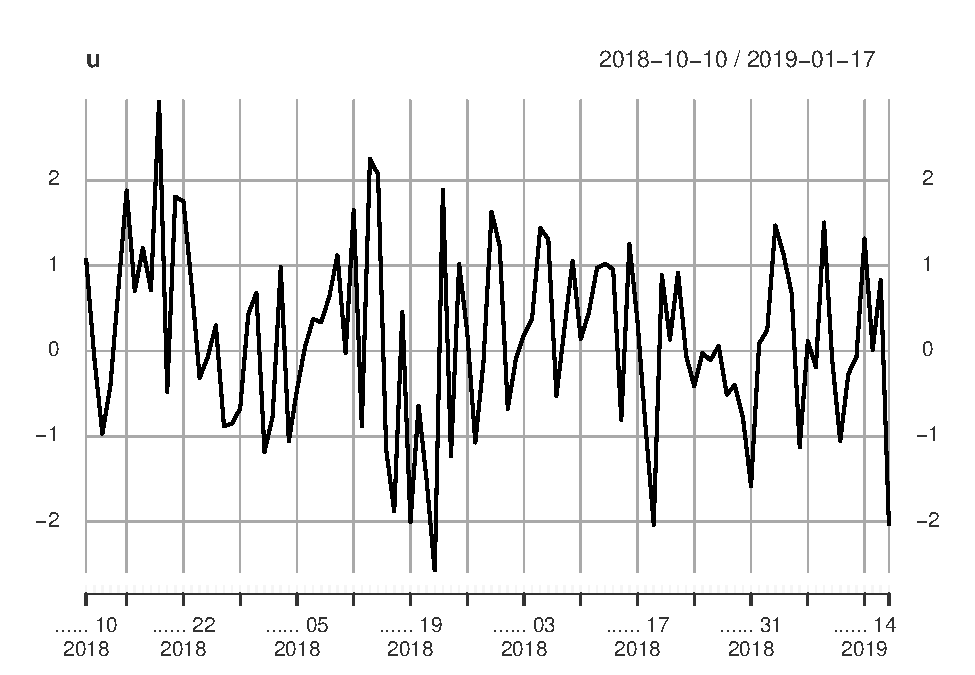
\includegraphics{timeseries2020_files/figure-latex/unnamed-chunk-2-1.pdf}

\begin{Shaded}
\begin{Highlighting}[]
\KeywordTok{mean}\NormalTok{(u)}
\end{Highlighting}
\end{Shaded}

\begin{verbatim}
## [1] 0.1497983
\end{verbatim}

\[
X \sim N(\mu, \sigma^2)\\
\text{ roughly } 95\% \text{ of the realisations of X are expected to be in the interval} \\
[\mu - 2\sigma, \mu + 2\sigma] 
\]

\[
X \sim N(0, 1)\\
[ - 2, 2]
\]

\begin{Shaded}
\begin{Highlighting}[]
\NormalTok{uL1 <-}\StringTok{ }\KeywordTok{lag}\NormalTok{(u)}
\NormalTok{combinedSeries <-}\StringTok{ }\KeywordTok{cbind}\NormalTok{(u, uL1)}
\KeywordTok{plot}\NormalTok{(}\KeywordTok{as.data.frame}\NormalTok{(uL1)[, }\DecValTok{1}\NormalTok{], }\KeywordTok{as.data.frame}\NormalTok{(u)[, }\DecValTok{1}\NormalTok{], }\DataTypeTok{xlab =} \StringTok{"u_\{t - 1\}"}\NormalTok{, }\DataTypeTok{ylab =} \StringTok{"u_\{t\}"}\NormalTok{, }\DataTypeTok{main =} \StringTok{"Scatterplot of u_t and u_\{t - 1\}"}\NormalTok{)}
\end{Highlighting}
\end{Shaded}

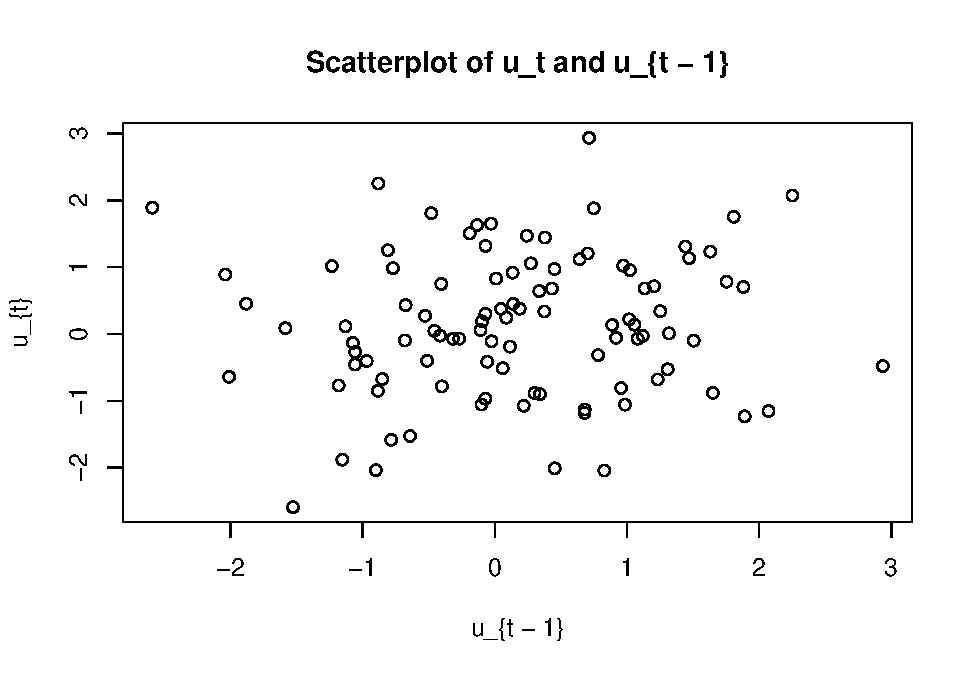
\includegraphics{timeseries2020_files/figure-latex/unnamed-chunk-3-1.pdf}

\begin{Shaded}
\begin{Highlighting}[]
\KeywordTok{hist}\NormalTok{(}\KeywordTok{as.data.frame}\NormalTok{(u)[, }\DecValTok{1}\NormalTok{], }\DataTypeTok{main =} \StringTok{"Histogram of u"}\NormalTok{)}
\end{Highlighting}
\end{Shaded}

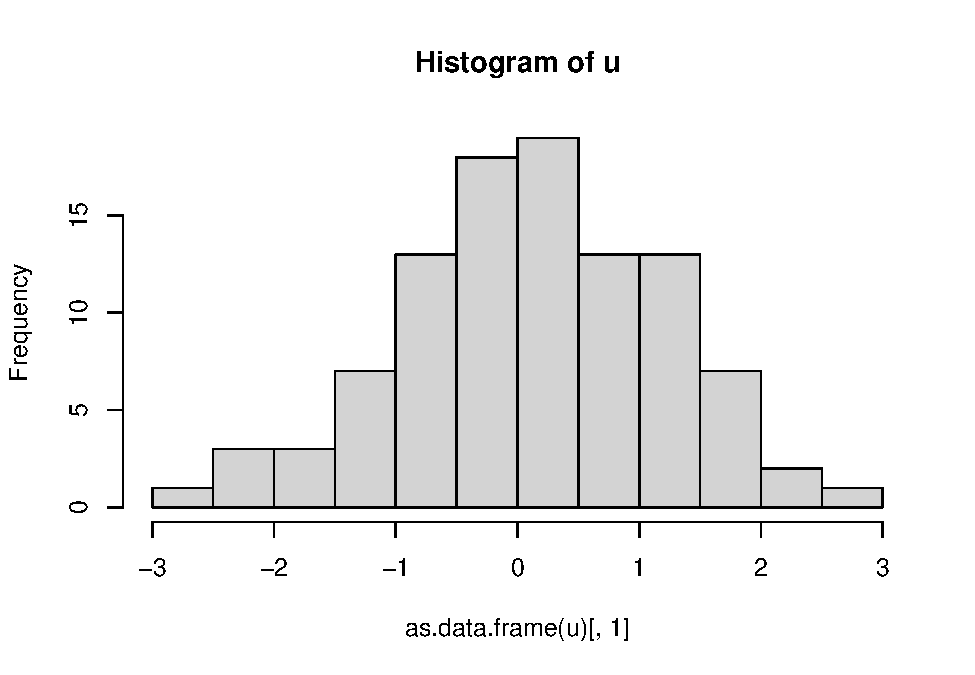
\includegraphics{timeseries2020_files/figure-latex/unnamed-chunk-4-1.pdf}

\hypertarget{sample-empirical-covariance}{%
\section{Sample (empirical) covariance}\label{sample-empirical-covariance}}

Let \(x\) and \(y\) be two random variables with \(T\) realisations.
\[
x: x_{1}, x_{2}, \ldots, x_{T}\\
y: y_{1}, y_{2}, \ldots, y_{T}\\
\]

\hypertarget{expected-value-of-y_t}{%
\section{\texorpdfstring{Expected value of \(y_t\)}{Expected value of y\_t}}\label{expected-value-of-y_t}}

\[
E(y_t) = E(x_t + 7u_t) = E(x_t) + E(7u_t) = x_{t} + E(7u_t) = x_{t} + 7\underbrace{E(u_t)}_{0} = x_t \\
E(y_t) = x_t \\
Var(7u_t) = 7^2 \underbrace{Var(u_t)}_{1} = 49
\]

\[
E(y_t) = \underbrace{E(x_t)}_{x_t} + \underbrace{E(7u_t)}_{0} \\
E(u_t) = 0 \text{ by the definition of the normal distribution with mean 0} \\
E(7u_t) = 7E(u_t) = 0 \text{ because 7 is a constant (non-random)}\\
Var(7u_t) = 7^2Var(u_t) = 7^2\times 1
\]

\begin{Shaded}
\begin{Highlighting}[]
\NormalTok{x <-}\StringTok{ }\DecValTok{1}\OperatorTok{:}\DecValTok{50}
\NormalTok{noise <-}\StringTok{ }\DecValTok{20}\OperatorTok{*}\KeywordTok{rnorm}\NormalTok{(}\DecValTok{50}\NormalTok{)}
\end{Highlighting}
\end{Shaded}

\begin{Shaded}
\begin{Highlighting}[]
\NormalTok{y <-}\StringTok{ }\DecValTok{100} \OperatorTok{*}\StringTok{ }\NormalTok{x }\OperatorTok{+}\StringTok{ }\NormalTok{noise}
\end{Highlighting}
\end{Shaded}

\[
E(y_t) = E(x_t + u_t) = E(x_{t}) + \underbrace{E(u_{t})}_{0} = E(x_t)
\]

\begin{Shaded}
\begin{Highlighting}[]
\KeywordTok{plot}\NormalTok{(x, y)}
\KeywordTok{mean}\NormalTok{(x)}
\end{Highlighting}
\end{Shaded}

\begin{verbatim}
## [1] 25.5
\end{verbatim}

\begin{Shaded}
\begin{Highlighting}[]
\KeywordTok{mean}\NormalTok{(y)}
\end{Highlighting}
\end{Shaded}

\begin{verbatim}
## [1] 2551.746
\end{verbatim}

\begin{Shaded}
\begin{Highlighting}[]
\KeywordTok{abline}\NormalTok{(}\DataTypeTok{v =} \KeywordTok{mean}\NormalTok{(x), }\DataTypeTok{col =} \DecValTok{3}\NormalTok{, }\DataTypeTok{lwd =} \DecValTok{2}\NormalTok{)}
\KeywordTok{abline}\NormalTok{(}\DataTypeTok{h =} \KeywordTok{mean}\NormalTok{(y), }\DataTypeTok{col =} \DecValTok{2}\NormalTok{, }\DataTypeTok{lwd =} \DecValTok{2}\NormalTok{)}
\end{Highlighting}
\end{Shaded}

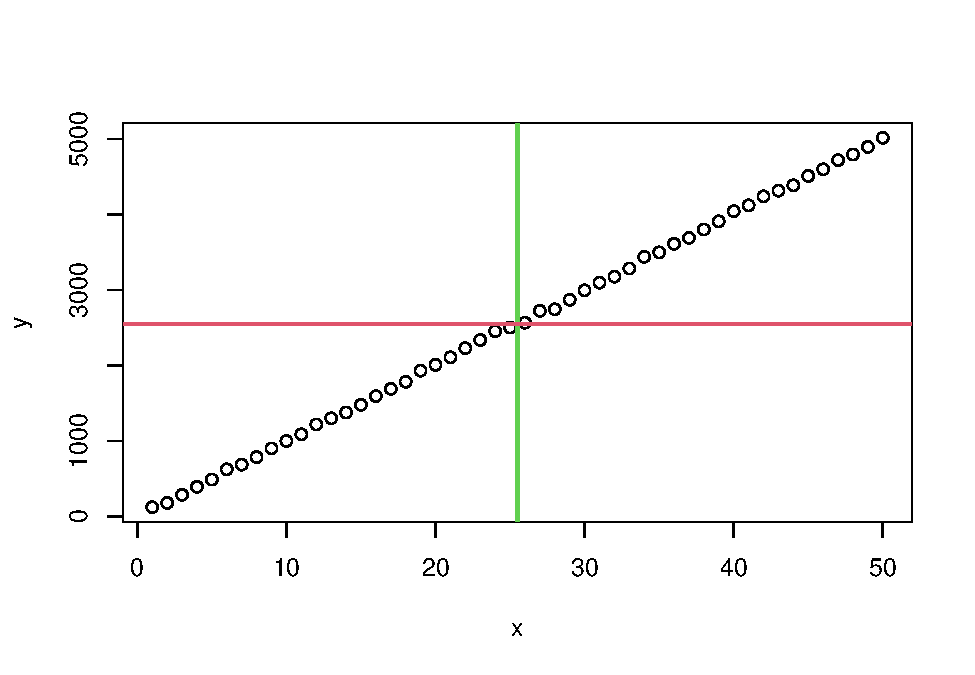
\includegraphics{timeseries2020_files/figure-latex/unnamed-chunk-7-1.pdf}

\begin{Shaded}
\begin{Highlighting}[]
\KeywordTok{cov}\NormalTok{(x, y)}
\end{Highlighting}
\end{Shaded}

\begin{verbatim}
## [1] 21331.89
\end{verbatim}

\[
(x_t - \overline{x})(y_{t} - \overline{y}) > 0 \text{ for points in the top right part}\\
(x_t - \overline{x})(y_{t} - \overline{y}) > 0 \text{ for points in the bottom left part}\\
(x_t - \overline{x})(y_{t} - \overline{y}) < 0 \text{ for points in the bottom right and top left parts}
\]
The sample covariance is defined as:
\[
Cov(x, y) = \frac{1}{T - 1}\sum_{t = 1}^{T}(x_t - \overline{x})(y_{t} - \overline{y})
\]

\[
\overline{y} = \frac{1}{T}\sum_{t = 1}^{T}y_{t} \\
(y_t - \overline{y}) > 0 \text{ for points above the red line}\\
(y_t - \overline{y}) < 0 \text{ for points below the red line}\\
(x_t - \overline{x}) > 0 \text{ for points to the right of the green line}\\
(x_t - \overline{x}) < 0 \text{ for points to the left of the green line}
\]

\$\$
s\^{}2(x) = \frac{1}{T - 1}\sum\emph{\{t = 1\}\^{}\{T\}(x\_t - \overline{x})\textsuperscript{2\textbackslash{}
s}2(y) = \frac{1}{T - 1}\sum}\{t = 1\}\^{}\{T\}(y\_t - \overline{y})\^{}2\textbackslash{}

\rho(x, y) = \frac{Cov(x, y)}{\sqrt{s^2(x)s^2(y)}} \text{ correlation coefficient}\textbackslash{}
-1 \leq \rho(x, y) \leq 1
\$\$

\[
y_{t} =  - x_{t}
\]

\[
\rho(x, y) = \rho(x, x) = \frac{Cov(x, x)}{\sqrt{s^2(x)s^2(x)}} = \frac{s^2(x)}{s^2(x)} = 1
\]

\[
Cov(x, x) = \frac{1}{T - 1}\sum_{t = 1}^{T}(x_t - \overline{x})^2 = Var(x) = s^2(x)
\]
\[
y_t = bx_{t} + a, \quad b,a \in R\\
b > 0: \rho(x, y) = 1\\
b < 0: \rho(x, y) = -1 \\
\]

\[
y_t, y_{t - 1}, y_{t - 2},\ldots, y_{t - k}
\]

\[
\gamma_0 = Cov(y_t, y_{t}) = Var(y_t) = s^2(x)\\
\gamma_{1} = Cov(y_{t}, y_{t - 1}) \text{ first order autocovariance }\\
\gamma_{2} = Cov(y_{t}, y_{t - 2}) \text{ second order autocovariance } \\
\gamma_{3} =Cov(y_{t}, y_{t - 3}) \text{ third order autocovariance } \\
\vdots \\
\gamma_{k} =Cov(y_{t}, y_{t - k}) \text{ k-th order autocovariance } \\
\]
\[
\rho_{0}= \rho(y_t, y_{t}) = 1 \\
\rho_{1} = \rho(y_{t}, y_{t - 1}) \text{ first order autocorrelation }\\
\rho_{2} = \rho(y_{t}, y_{t - 2}) \text{ second order autocorrelation } \\
\rho_{3} =\rho(y_{t}, y_{t - 3}) \text{ third order autocorrelation } \\
\vdots \\
\rho_{k} =\rho(y_{t}, y_{t - k}) \text{ k-th order autocorrelation } \\
\]

\[
\rho_1 = \frac{\gamma_1}{\gamma_0} \\
\rho_2 = \frac{\gamma_2}{\gamma_0} \\
\vdots\\
\rho_k = \frac{\gamma_k}{\gamma_0}\\
\]
\[
\text{Assume that } s^2(y_t) = s^2(y_{t - 1}) \\
\rho_{1} = \rho(y_t, y_{t - 1}) = \frac{Cov(y_t, y_{t - 1})}{\sqrt{s^2(y_t)s^2(y_{t})}} = \frac{Cov(y_t, y_{t - 1})}{s^2(y_t)} = \frac{\gamma_1}{\gamma_0}
\]

\[
u_t \sim N(0, 1) \\
u_{t} \text{ and } u_{t - k} \text{ are not correlated for each } k \neq 0.
\]

\hypertarget{exercise}{%
\section{Exercise}\label{exercise}}

Compute the sample first order autocovariance of the following time series.

\$\$
x: x\_1, x\_2, x\_3\textbackslash{}
x: (2, 3, 10)\textbackslash{}

Cov(x\_t, x\_\{t - 1\}) = \frac{1}{T - 1}\sum\emph{\{t = 1\}\^{}\{T\}(x\_t - \overline{x})(x}\{t - 1\} - \overline{x})\textbackslash{}
\overline{x} = 5\textbackslash{}
\gamma\emph{1 = Cov(x\_t, x}\{t - 1\}) = \frac{1}{3 - 1}{[}(2 - 5)(NA - 5) + (3 - 5)(2 - 5) + (10 - 5)(3 - 5){]} =\textbackslash{}
= \frac{1}{2}{[}NA + (-2)(-3) + (5)(-2){]} = \frac{1}{2}(6 -10) = -2\textbackslash{}
\gamma\emph{1 = -2\textbackslash{}
\rho}\{1\} = ? \textbackslash{}

s\^{}2(x) = Var(x\_\{t\}) = \frac{1}{T - 1}\sum\_\{t = 1\}\^{}\{T\}\left[(x_t - \overline{x})^2\right] =\textbackslash{}
\frac{1}{3 - 1}{[}(2 - 5)\^{}2 + (3 - 5)\^{}2 + (10 - 5)\^{}2{]} = \frac{1}{2}{[}(-3)\^{}2 + (-2)\^{}2 + 5\^{}2{]} = \textbackslash{}
\frac{1}{2}{[}9 + 4 + 25{]} = \frac{38}{2} = 19\textbackslash{}
\gamma\emph{0 = 19\textbackslash{}
\rho}\{1\} = \frac{\gamma_1}{\gamma_0} = \frac{-2}{19} = \ldots{}
\$\$

  \bibliography{bibliography.bib,packages.bib}

\end{document}
